% Draft for paper 1's journal version (arXiv v2), hardening plan Phase 3, 10 Nov 2026. Not included in the arXiv v1
% source. Every number is a macro of experiments/results/break_even/be_metrics.tex (evaluation/break_even_rule.py);
% the figure is paper/figures/break_even_map.pdf from the same script. To include: \input the macro file in the
% preamble and this file after the learned-bottleneck section. Jointly trained codes added 11 Nov 2026 (run 2,
% experiments/results/joint_bottleneck/, evaluation/joint_bottleneck.py). Revised after an independent audit
% (11 Nov 2026): speed scaling corrected, the check called a consistency check, the survey scoped to the conditions it
% tests, grid resolution and sample sizes given, the JPEG grid and the training asymmetry stated.
\subsection{When can a split pay off? A design rule}\label{sec:design-rule}
Proposition~\ref{prop:dominance} settles splits that need at least an image's bits, onboard time and onboard-plus-server
time. Learned codes are smaller, so we ask where, in onboard speed and goodput, \emph{any} code can beat every
measured JPEG setting. In the model of Section~\ref{sec:model}, an option $c$ has onboard time $e_c$, payload $b_c$,
server time $s_c$, accuracy $A_c$, frame rate $F/\lceil F\max(e_c, b_c/B)\rceil$, and on-time probability
$p_c(B) = Q\big((R_c - B)/\sigma(B)\big)$, where $Q$ is the standard normal tail, $R_c = b_c/(D - e_c - d - s_c)$ is the
required rate, and the goodput spread is $\sigma(B) \le sB$ for every option.

\begin{proposition}[Break-even goodput against the image family]\label{prop:be-family}
Let $m_k = \max(e_k, 1/F)$ for a split code $k$, and fix $P<1$ with normal quantile $z_P$ and $z_P s < 1$. An image
setting $q$ with $P A_q \ge A_k$ and $e_q \le m_k$ gives $U_q(B) \ge U_k(B)$ whenever
$B \ge \max\big(b_q/m_k,\; R_q/(1 - z_P s)\big)$. Hence $k$ can beat every image setting only below
\begin{equation*}
B_{\mathrm{be}}(k) = \min_{q:\,P A_q \ge A_k,\; e_q \le m_k} \max\Big(\frac{b_q}{m_k},\; \frac{R_q}{1 - z_P s}\Big),
\end{equation*}
with $B_{\mathrm{be}} = \infty$ if no setting qualifies.
\end{proposition}
\begin{proof}
From $b_q \le B m_k$ and $e_q \le m_k$:
\begin{align*}
\lceil F\max(e_q, b_q/B)\rceil &\le \lceil F m_k\rceil = \max(1, \lceil F e_k\rceil)\\
&\le \lceil F\max(e_k, b_k/B)\rceil ,
\end{align*}
so $f_q \ge f_k$. Since $\sigma(B) \le sB$, $B \ge R_q/(1 - z_P s)$ gives $p_q \ge P$. Hence
$U_q \ge P f_q A_q \ge f_k A_k \ge U_k$.
\end{proof}
\noindent The first term, $b_q/m_k$, grows with onboard speed: a faster device shortens $e_k = t_{\mathrm{full}}(\phi_k +
\rho_k)$, so a code can win at higher goodputs. The growth stops where the camera rate binds ($m_k = 1/F$), or where the
deadline term $R_q/(1 - z_P s)$ dominates.

\begin{figure}[t]
\centering
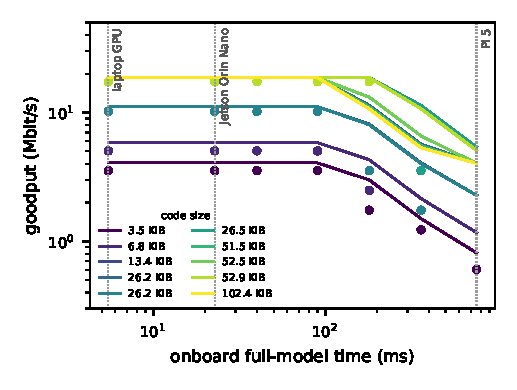
\includegraphics[width=\columnwidth]{figures/break_even_map.pdf}
\caption{Break-even goodput $B_{\mathrm{be}}$ of each learned code against the measured JPEG settings (lines,
Proposition~\ref{prop:be-family} with $P = \BePOn$) and the largest goodput at which the model of
Section~\ref{sec:model} has the code beat every one of them (dots). The x-axis is the onboard full-model time: the
paper's sweep and the three measured devices. Dashed lines and open dots: the same codes trained jointly with the
detector's server-side layers.}
\label{fig:break-even}
\end{figure}
\textbf{Consistency check.} We evaluated the \BeCodes{} learned codes (including the four jointly trained ones below) and
the post-hoc INT8 splits. The goodputs were those of Section~\ref{sec:learned}: a grid with steps of \BeGridStepPct\,\%.
The onboard speeds were \BeMeasuredDevices{} measured devices (the laptop GPU, the Jetson Orin Nano and the throttled
Pi~5) and \BeSweepSpeeds{} speeds of the paper's sweep. In the model, a split code beats the best JPEG setting in
\BeCells{} cells, and all of them lie below its $B_{\mathrm{be}}$ (\BeViolations{} exceptions). This check uses the
same model as the proposition, so it confirms the derivation and its implementation, not the model itself;
Section~\ref{sec:gen-mc} compares the model with the simulator.

\textbf{How close the bound is.}
\begin{itemize}
\item On the laptop and the Jetson, \BeTightFastN{} code--device pairs win at some goodput. Each one's largest winning
goodput is within \BeTightFastMax\,\% of $B_{\mathrm{be}}$, which is less than one grid step.
\item On the Pi, only \BePiWinCodesFrozen{} frozen code wins at all: the \BePiCodeKib~KiB code. The proposition limits
it to below \BePiBe~Mbit/s (against JPEG \BePiQstar), and it wins up to \BePiWin~Mbit/s.
\end{itemize}

\textbf{Post-hoc splits.} The \BeSurveyRows{} rows of the \BeSurveyModels-detector survey all meet the bit and onboard
conditions of Proposition~\ref{prop:dominance}: more bits and more onboard work than a Q95 JPEG. The server-time
condition was measured for YOLOv8s only; there it holds on any processor slower than about \GenDominanceTmin~ms per
full inference. For these detectors on such processors, a post-hoc split cannot exceed its accuracy ratio over the
image.

\textbf{Jointly trained codes.} We also trained the bottleneck together with the detector's server-side layers, on the
detection loss. This raised the accuracy of the \BeJointCodes{} codes by \BeJointGainMin{} to \BeJointGainMax{}
mAP$_{50:95}$ on the same held-out frames.
\begin{itemize}
\item The two smallest gains are below the bootstrap half-width of the estimates (up to \BeJointHalfCi), and we do not
claim them.
\item The gain is largest for the smallest code: at \BeJointPiCodeKib~KiB it reaches \BeJointSmallMap{}, against
\BeFrozenSmallMap{} when trained on the frozen detector.
\item The comparison favours the split. The split's server side gets extra training, while the image path keeps the
unmodified detector. A detector fine-tuned on low-quality JPEG would gain as well, so these gains bound the split's
advantage from above.
\end{itemize}
Higher accuracy moves $B_{\mathrm{be}}$ up, because a better JPEG setting is now needed to match it (\BeJointPiQstar{}
instead of \BePiQstar):
\begin{itemize}
\item on the Jetson, from \BeFrozenFastBe{} to \BeJointFastBe~Mbit/s, and the code wins up to \BeJointFastWin{} instead
of \BeFrozenFastWin~Mbit/s;
\item on the Pi, from \BePiBe{} to \BeJointPiBe~Mbit/s, and it wins up to \BeJointPiWin{} instead of
\BePiWin~Mbit/s;
\item on the Pi, the jointly trained \BeJointKtwoKib~KiB code at the second cut wins at one goodput,
\BeJointKtwoPiWin~Mbit/s, against $B_{\mathrm{be}} = \BeJointKtwoPiBe$; its frozen version never wins.
\end{itemize}
The \BeJointShift\,\% shift for the smallest code is partly an artefact of the JPEG grid. We measured \BeJpegQualities{}
qualities, so the matching setting jumps a whole step; the three lowest (Q10--Q35) also take the Q50 row's encode and
server times. Every winning cell of the jointly trained codes lies below its $B_{\mathrm{be}}$; they are included in
the \BeCells{} cells above. Joint training therefore widens the regime in which a split can pay off, but does not remove
its bound: above $B_{\mathrm{be}}$, the image wins.

\textbf{Design rule.} Before building a split, compute $B_{\mathrm{be}}$ from:
\begin{itemize}
\item the code's size and accuracy;
\item the JPEG rate--accuracy curve on the same frames;
\item the device's full-model time.
\end{itemize}
If the link's goodput is mostly above $B_{\mathrm{be}}$, send the image.
